\documentclass[handout]{beamer}
\usepackage{multicol}
\usepackage{xy}
\everymath{\displaystyle}
\mode<presentation>
{\usetheme{Warsaw}\setbeamercovered{dynamic}}
\usecolortheme{crane}
\usepackage{beamerfoils}
\pgfdeclareimage[height=1in]{university-logo}{ISULogo}
\logo{\pgfuseimage{university-logo}}
\setbeamertemplate{navigation symbols}{}
\title[\S6]{Section 6\\{\em And} and {\em or} problems}
\author{Dr Marcus Bishop}
\subject{Math 104}
\beamerdefaultoverlayspecification{<+->}
\theoremstyle{definition}
\newtheorem{remark}{Remark}
\newtheorem{impact}{Impact}
\newtheorem{notation}{Notation}
\usepackage{arev}
\begin{document}
\begin{frame}\titlepage\end{frame}
\LogoOff

\begin{frame}{Card problem from exam}
\begin{itemize}
\item How many cards either are picture cards or have
suit \alert{$\varheart$}?
\item Observe that thirteen cards have
suit \alert{$\varheart$}, namely
\[A\alert{\varheart},
2\alert{\varheart},
3\alert{\varheart},\ldots,
10\alert{\varheart},
J\alert{\varheart},
Q\alert{\varheart},
K\alert{\varheart}\]
\item Observe that twelve cards are picture cards, namely
\[J\alert{\varheart},J\alert{\vardiamond},J\clubsuit,J\spadesuit,
Q\alert{\varheart},Q\alert{\vardiamond},Q\clubsuit,Q\spadesuit,
K\alert{\varheart},K\alert{\vardiamond},K\clubsuit,K\spadesuit\]
\item However, \alert{three} cards in both groups,
namely
\[J\alert{\varheart},Q\alert{\varheart},K\alert{\varheart}\]
\item Thus $13+12-3=22$ cards are either picture cards or have 
suit \alert{$\varheart$}
\end{itemize}
\end{frame}

\begin{frame}{Inclusion-Exclusion Formula}
\begin{theorem}[Inclusion-Exclusion Formula]
Suppose that
\begin{itemize}
\item $M$ has $m$ elements 
\item $N$ has $n$ elements
\item There are $p$ elements in \alert{both} $M$ and $N$
\end{itemize}
Then there are $m+n-p$ elements in \alert{either} $M$ or $N$
\end{theorem}
\end{frame}

\begin{frame}{Example}
\begin{itemize}
\item How many of $1,2,\ldots,12$ are
either divisible by $3$ or greater than $6$?
\item Numbers divisible by $3$: $3,6,9,12$
\item Numbers greater than $6$: $7,8,9,10,11,12$
\item Numbers in both groups: $9,12$
\item Thus $4+6-2=8$
either divisible by $3$ or greater than $6$?
\end{itemize}
\end{frame}

\begin{frame}{Venn diagrams}
\begin{itemize}
\item Can visualize last example using Venn diagram:
\[\begin{xy}<1cm,0cm>:
(-1,0)*\cir<2cm>{};
(1,0)*\cir<2cm>{};
(-1.5,1)*{3};
(-1.5,-1)*{6};
(0,1)*{9};
(0,-1)*{12};
(1.25,1)*{7};
(1.25,-1)*{10};
(2,1)*{8};
(2,-1)*{11};
\end{xy}\]
\item Numbers divisible by $3$ in left circle
\item Numbers greater than $6$ in right circle
\item Numbers in both groups in both circles
\end{itemize}
\end{frame}

\begin{frame}{Greek, Roman, Russian alphabets}
\begin{multicols}{2}
\begin{itemize}
\item Upper left circle shows letters of Greek alphabet
\item Upper right circle shows letters of Roman alphabet
\item Lower circle shows letters of Russian alphabet
\item How many in Roman and Russian but not Greek?
\only<+->{One, namely C}
\item How many letters in all three?
\only<+->{11}
\end{itemize}
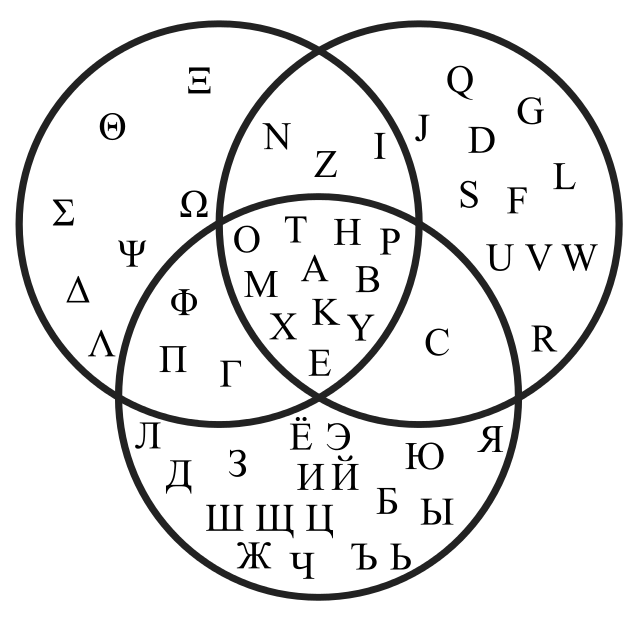
\includegraphics[scale=.25]{Venn}
\end{multicols}
\end{frame}

\begin{frame}{Freshman music majors}
\begin{itemize}
\item $100$ freshman majoring in (instrumental) music
required to be in either band or orchestra
\item $75$ in band
\item $35$ in both band and orchestra
\item How many in orchestra?
\item Rather than drawing freshmen in circles,
write only \alert{number} of freshman in each
group in corresponding circle
\[\begin{xy}<1cm,0cm>:
(-1,2)*+!D{\text{Band}};
(1,2)*+!D{\text{Orch}};
(-1,0)*\cir<2cm>{};
(1,0)*\cir<2cm>{};
(0,0)*{35};
\end{xy}\]
\end{itemize}
\end{frame}

\begin{frame}
\begin{itemize}
\item Since $75$ in band, must have
$40$ in band but not orchestra:
\[\begin{xy}<1cm,0cm>:
(-1,2)*+!D{\text{Band}};
(1,2)*+!D{\text{Orch}};
(-1,0)*\cir<2cm>{};
(1,0)*\cir<2cm>{};
(0,0)*{35};
(-2,0)*{40};
\end{xy}\]
\end{itemize}
\end{frame}

\begin{frame}
\begin{itemize}
\item Must be $100-75=25$ in orchestra but not band:
\[\begin{xy}<1cm,0cm>:
(-1,2)*+!D{\text{Band}};
(1,2)*+!D{\text{Orch}};
(-1,0)*\cir<2cm>{};
(1,0)*\cir<2cm>{};
(0,0)*{35};
(-2,0)*{40};
(2,0)*{25};
\end{xy}\]
\item Thus $40+25=65$ in orchestra
\end{itemize}
\end{frame}

\end{document}
